\documentclass[conference,9pt]{IEEEtran}
\IEEEoverridecommandlockouts

\usepackage{cite}
\usepackage{amsmath,amssymb,amsfonts}
\usepackage{graphicx}
\usepackage{textcomp}
\usepackage{xcolor}
\usepackage{booktabs}
\usepackage{algorithm}
\usepackage{algpseudocode}
\usepackage{tikz}
\usetikzlibrary{arrows.meta,positioning,shapes.geometric}
\usepackage{pgfplots}
\pgfplotsset{compat=1.18}
\usepackage{listings}
\usepackage{caption}
\usepackage{subcaption}
\usepackage{microtype}
\usepackage{placeins}
\usepackage[hidelinks]{hyperref}
\usepackage{float}

\captionsetup[figure]{justification=centering,singlelinecheck=true,labelsep=period}

\graphicspath{{figures/}}

\lstdefinelanguage{json}{
    basicstyle=\ttfamily\scriptsize,
    showstringspaces=false,
    breaklines=true,
    frame=single,
    literate=
     *{0}{{{\color{blue}0}}}{1}
      {1}{{{\color{blue}1}}}{1}
      {2}{{{\color{blue}2}}}{1}
      {3}{{{\color{blue}3}}}{1}
      {4}{{{\color{blue}4}}}{1}
      {5}{{{\color{blue}5}}}{1}
      {6}{{{\color{blue}6}}}{1}
      {7}{{{\color{blue}7}}}{1}
      {8}{{{\color{blue}8}}}{1}
      {9}{{{\color{blue}9}}}{1}
}

\begin{document}

\title{Zero-Touch Federated Learning Attacks with an LLM-Directed\\ Reinforcement-Learning Attacker}

\author{
\IEEEauthorblockN{
Pasindu Mallawarachchi$^{*}$, Isuru Madusanke$^{\dagger}$, Tharushika Nettasinghe$^{\ddagger}$, Dinuth Kumara$^{\S}$,\\
Chamara Sandeepa$^{\P}$, Tharindu Gamage$^{\|}$, Madhusanka Liyanage$^{**}$
}
\IEEEauthorblockA{
$^{*\dagger\ddagger\S\|}$Faculty of Engineering, University of Ruhuna, Sri Lanka\\
$^{\P **}$Network Softwarization and Security Labs (NetsLab), School of Computer Science, University College Dublin, Ireland\\
$^{*}$imalsha\_map\_e23@engug.ruh.ac.lk,
$^{\dagger}$kumara\_armdd\_e23@engug.ruh.ac.lk,
$^{\ddagger}$nettasinghe\_tn\_e22@engug.ruh.ac.lk,\\
$^{\S}$kumara\_dk\_e22@engug.ruh.ac.lk\\
$^{\P}$abeysinghe.sandeepa@ucd.ie,
$^{\|}$tharindu@eie.ruh.ac.lk,
$^{**}$madhusanka@ucd.ie
}
}

\maketitle

\begin{abstract}
Federated learning (FL) aggregates client model updates without inspecting the raw client data, which gives the central server no immediate way to verify whether a submitted update corresponds to honest training. We propose a zero touch FL attacker, an LLM policy trained with Group Relative Policy Optimization (GRPO) that autonomously decides which of its controllable clients to poison in each round, and generates an ordered plan of primitive weight space operators for each selected client. The plan generated is executed by a deterministic interpreter on the honest update of a client, instead of the LLM updating the model weights directly.
The policy is trained with a single verifiable continuous reward that rewards induced accuracy loss and evasion of a training time detector, penalized for malformed output, unnecessary client use and near duplicate Sybil like collusion when multiple clients are used together. We assess the both trained and frozen attacker by replaying its committed actions unmodified against four independently evolving, fixed server- side defenses FLTrust, Multi Krum, DnC and DeFL. Through two poison budget regimes, a strict minority of controllable clients and a coalition spanning half of the federation. Finally, these defenses are used only as external benchmarks to evaluate the transferability of the learned attack.

\end{abstract}

\begin{IEEEkeywords}
federated learning, model poisoning, large language models, reinforcement learning, Group-Relative Policy Optimization, Byzantine-robust aggregation, adversarial machine learning, autonomous attackers
\end{IEEEkeywords}

\section{Introduction}

Federated learning (FL) allows edge devices to collaboratively train a shared model without revealing local data \cite{fedavg}. In each round, a central server distributes the global model across all clients, each client performs local training, and the server aggregates the returned updates, typically via Federated Averaging (FedAvg) into a new global model. The server only sees model updates, and thus has no independent implies to verify that a particular update is the result of honest training. A subset of compromised clients can submit manipulated updates that degrade the accuracy of the global model \cite{bagdasaryan2020,bhagoji2019}. Existing attack studies mostly hand-design the attacker a set of rules to determine which clients to corrupt and a fixed formula to alter their updates \cite{fang2020,xie2020fallofempires,baruch2019little}. 

Instead we ask whether an attacker can learn end-to-end from interaction. An LLM policy only observes dimensionless statistics of its own controllable clients’ honest updates, no cross-client reference and no defense internals, and needs to decide, every round, which clients to poison and how. It produces a small domain-specific-language (DSL) plan of primitive weight operators which is consumed by a deterministic interpreter so the policy never sees raw weights directly. We train this policy with GRPO \cite{grpo} on a single verifiable reward that combines accuracy degradation, evasion of training-time detector, output validity, client-budget efficiency, and diversity across jointly poisoned clients.

 To evaluate for generalization of the resulting strategy, we freeze the trained attacker and replay its committed action unmodified against four fixed server-side defenses, each evolving its own global model independently. The defenses are not designed in this paper, but are rather used as external benchmarks to test the attacker. This isolates the defense as the only variable in the comparison. It tests transfer to defenses the attacker never trained against.n the comparison and tests transfer to defenses the attacker never trained against.

\textbf{Contributions.} This paper makes the following contributions:
\begin{itemize}
    \item A zero-touch FL attacker in which client selection and weight-operator composition are generated directly by an LLM policy, over a general-purpose primitive-operator DSL, without prescribing any attack strategy in advance.
    \item A verifiable, continuous reward that jointly credits accuracy degradation and evasion while penalizing malformed output, the use of more controllable clients than necessary, and non-diverse (Sybil-like) multi-client collusion, computed from ground truth available only during training.
   \item A GRPO training strategy with stochastic opponent scoring and an opponent league to keep the attacker's learning signal alive against an evolving, a non-deterministic detector avoiding the zero-advantage collapse that a small, near-binary action space is prone to experience.
    \item A \emph{fixed-attack, varied-defense benchmark harness} that replays one committed attack plan per round against four independently evolving, defenses across two poison-budget regimes, testing whether the learned evasion strategy transfers to defenses never seen during training.
    \item An open system design covering the attacker contract, reward, training schedule, and benchmark protocol, forming a reusable testbed for studying autonomous, LLM-directed FL attacks.
\end{itemize}

The remaining sections cover related work, the threat model, the attack mechanism, GRPO training, the experimental setup, results, limitations, and future work.

\section{Related Work}
\label{sec:related}

\subsection{Federated Learning and the Poisoning Attack Surface}
In a standard FL round, a central server distributes the global model to $N$ clients, each performs local training, and the server aggregates the returned updates through FedAvg \cite{fedavg}. Model poisoning occurs when compromised clients submit manipulated updates. Untargeted attacks degrade overall accuracy, whereas targeted backdoor attacks introduce a narrower vulnerability while leaving overall accuracy largely intact \cite{bagdasaryan2020,wang2020attackoftails}. This paper focuses on reducing the global model's overall test accuracy while evading detection. Non-IID data partitioning makes detection harder because an honest client's update can legitimately differ from the majority.

\subsection{Byzantine-Robust and Statistical Defenses}
Coordinate-wise median and trimmed-mean aggregation bound the influence of individual coordinates \cite{byzantine}. Krum and Multi-Krum retain updates that are close to their neighbors under Euclidean distance \cite{krum}. DnC centers the updates, projects them onto the leading right singular vector, and removes clients with large projections \cite{dnc}. FLTrust derives a trusted direction from a clean server dataset and forms a cosine-weighted average \cite{fltrust}. FoolsGold reduces the weight of clients with similar contribution histories \cite{foolsgold}. DeFL tracks layer-wise gradient norms and applies an adaptive outlier vote during critical learning periods \cite{defl}. FLAME clusters client updates and combines adaptive clipping with noise injection to remove backdoor contributions while bounding accuracy loss \cite{nguyen2022flame}. Each method relies on a fixed geometric or statistical prior; Section~\ref{sec:defense-panel} uses four such defenses, none of which the attacker studied here trains against, purely as evaluation targets.

\subsection{Adaptive and Learning-Based Attacks}
A defense-aware attacker can construct updates that satisfy a robust aggregator's assumptions while still corrupting the result. Fang~et~al.\ optimize local model poisoning against known aggregation rules \cite{fang2020}. Bhagoji~et~al.\ show that one persistent attacker using boosted updates can bias the global model \cite{bhagoji2019}. Xie~et~al.\ manipulate the inner product between the aggregate and the true gradient to slip past distance-based screens \cite{xie2020fallofempires}, and Baruch~et~al.\ show that small, carefully bounded perturbations from several colluding clients (``a little is enough'') can evade defenses tuned to catch large outliers \cite{baruch2019little}. Wang~et~al.\ target rare data subpopulations to plant durable backdoors \cite{wang2020attackoftails}, and Cao and Gong fabricate fake client identities entirely (an orthogonal, Sybil attack surface we do not model here) \cite{cao2022mpaf}. Unlike this body of work, our attacker receives no closed-form knowledge of the aggregation rule and no white-box access to defense parameters, thresholds, or scores; it learns a policy purely from interaction outcomes.

\subsection{Reinforcement Learning of LLM Policies}
GRPO samples $G$ completions per state, assigns each a verifiable reward, and normalizes rewards within the group to obtain the policy advantage without a separate critic network \cite{grpo}, building on the clipped policy-gradient framework of Proximal Policy Optimization (PPO) \cite{schulman2017ppo} and on RLHF-style fine-tuning of instruction-following LLMs \cite{ouyang2022instructgpt}. GRPO fits our setting because each attack round produces one terminal, exactly computable reward. Low-Rank Adaptation (LoRA) provides a small trainable adapter over one shared, frozen base model \cite{lora2022}; we use the open-weight Llama-3.2 family as that base \cite{dubey2024llama3}.

\section{Threat Model}
\label{sec:threat}

\textbf{Problem statement.} Recent FL security researches usually assume a fixed attack against a fixed defense. This cannot discover automatically a new attack when the defense changes, adapting the attack requires a human to design another strategy. We aim to replace this fixed high-level strategy with a learned approach: In round $t$, implementing an attacker policy $\pi_A$  observes $o_t^A$ from its clients’ honest updates and outputs an action $a_t$ with a client selection and an ordered weight-operation plan.

\begin{equation}
\max_{\pi_A}\;\mathbb{E}[R_{\mathrm{att}}].
\label{eq:agentic_problem}
\end{equation}

The policy optimizes a verifiable reward by repeated interaction with the FL environment, the environment offers a fixed set of primitive operators and a fixed communication interface, but no fixed attack template or client selection rule is provided. We use a \emph{partial-insider} threat model for this policy.

\textbf{Attacker capabilities.} The attacker controls and poisons a fixed number of clients (5 or 10, out of $N=20$, depending on the run) in every round across the entire run. For each of these controlled clients, the attacker observes per-layer statistics of that client's \emph{own honest update} relative to the current global model (Section~\ref{sec:attacker-contract}). It does not receive a robust reference such as the coordinate-wise median, another client's update, or a statistic computed over the run. The attacker cannot alter the server's aggregation code or inject clients outside its fixed clients, and it cannot see any defense's internal state (features, thresholds, trust scores, or verdicts) at training or evaluation time.

\textbf{Defense visibility.} During training, the attacker reward depends only on the global-model accuracy and a scalar confidence value returned by a training-time detector opponent (Section~\ref{sec:rewards}); its prompt never contains per-client features of that detector. A frozen attacker’s committed action is replayed unmodified at evaluation time against each benchmark defense (Section~\ref{sec:defense-panel}). The attacker never responds or otherwise trains against the internal state of any classical defense in the panel, so damage measured under those defenses is a reflection of transfer rather than direct co-adaptation.

\textbf{Out of scope.} We do not model network-level attacks, Sybil attacks that fabricate new client identities \cite{cao2022mpaf}, data-poisoning attacks mounted at a client's local training data, targeted/backdoor objectives, or collusion with a compromised aggregation server. These are natural extensions of the testbed (Section~\ref{sec:conclusion}) but are not evaluated here.

\begin{figure}[t]
\centering
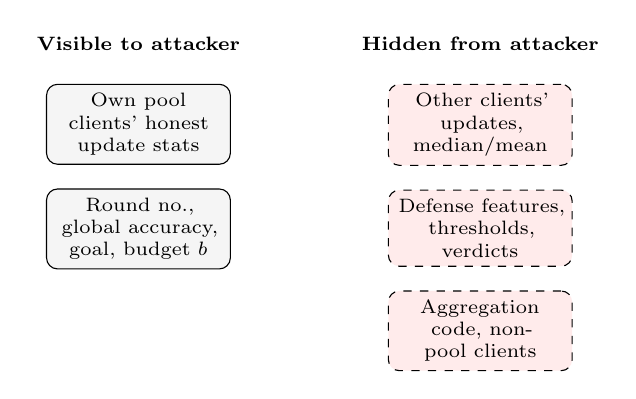
\begin{tikzpicture}[
    node distance=0.3cm and 0.4cm,
    every node/.style={font=\scriptsize},
    box/.style={draw, rounded corners, align=center, minimum height=0.6cm, text width=2.1cm, fill=gray!8},
    hidebox/.style={draw, rounded corners, align=center, minimum height=0.6cm, text width=2.1cm, fill=red!8, dashed},
    lbl/.style={font=\scriptsize\bfseries}
]
\node[lbl] (vislbl) {Visible to attacker};
\node[box, below=of vislbl] (v1) {Own pool clients' honest update stats};
\node[box, below=of v1] (v2) {Round no., global accuracy, goal, budget $b$};

\node[lbl, right=1.3cm of vislbl] (hidlbl) {Hidden from attacker};
\node[hidebox, below=of hidlbl] (h1) {Other clients' updates, median/mean};
\node[hidebox, below=of h1] (h2) {Defense features, thresholds, verdicts};
\node[hidebox, below=of h2] (h3) {Aggregation code, non-pool clients};
\end{tikzpicture}
\caption{Partial-insider observability boundary.}
\vspace{2mm}
\small \textit This boundary shows what the attacker's policy can and cannot see, at both training and evaluation time.
\label{fig:threatmodel}
\end{figure}
Figure~\ref{fig:threatmodel} summarizes this observability boundary.

\section{Attacker Design}
\label{sec:attack}

\subsection{Model and Data Environment}
The environment simulates FL across three datasets (Fashion MNIST, MNIST, and 5G-NIDD) with varying total client sizes of $N \in \{5, 10, 20\}$. Data is distributed under a non-IID partition using the FLTrust-style bias-$q$ scheme, in which each client's local data is skewed toward a subset of classes with bias strength $q$ \cite{fltrust}. The global model is a lightweight multilayer perceptron (MLP) with 970 parameters (\texttt{AvgPool2d(4)} $\to$ \texttt{Linear(49,16)} $\to$ \texttt{ReLU} $\to$ \texttt{Linear(16,10)}). At this scale, per-layer statistics provide a compact observation an LLM can process as structured JSON rather than raw tensors, while the model still contains distinct weight and bias tensors the attacker can target selectively.

Initially, $N$ clients train honestly using FedAvg for a fixed number of rounds. The resulting global model, the per-client weights, and the baseline accuracy are checkpointed and form the initial state for each attack round that follows. From that point, the attacker interacts with the environment in each round: it chooses and poisons clients, the server aggregates the accuracy and detector feedbacks (training only) are used to drive the reward as described in Section~\ref{sec:rewards}.

\subsection{Attacker Contract}
\label{sec:attacker-contract}
\textbf{Input.} The attacker observes the round number, current global accuracy, an attack goal (\texttt{untargeted\_degrade}, evaluated in this paper, lower global test accuracy by a target amount), the controllable client pool $P$, and round budget $b$. For each pool client's honest update $\Delta = \mathrm{local} - \mathrm{global}$, the observation includes relative update norm $\|\Delta\|/\|G\|$, RMS delta, energy fraction, sign-flip fraction, standard-deviation ratio, absolute-mean ratio, and whole-model cosine similarity to the global model. These are normalized only against the global model; median, mean, and cross-client references remain unavailable to the partial insider. This representation is dimensionless, architecture independent, and unaffected by the round budget. Table~\ref{tab:input_stats} summarizes these statistics.


\begin{table}[!ht]
\caption{Client-specific input statistics provided to the attacker.}
\label{tab:input_stats}
\centering
\small
\begin{tabular}{@{}p{1.8cm}p{3.0cm}p{3.2cm}@{}}
\toprule
\textbf{Statistic} & \textbf{Equation} & \textbf{Purpose} \\
\midrule
Relative update norm & $\|\Delta\| / \|G\|$ & Measures update magnitude relative to the global model size. \\
RMS delta & $\|\Delta\| / \sqrt{N}$ & Average step size for an individual weight in the layer. \\
Energy fraction & $\|\Delta_{\mathrm{layer}}\|^2 / \|\Delta_{\mathrm{model}}\|^2$ & Proportion of the client's total update concentrated in this layer. \\
Sign-flip fraction & $\frac{1}{N} \sum \mathbf{1}(\mathrm{sign}(C) \neq \mathrm{sign}(G))$ & Fraction of weights that flipped their sign. \\
Standard-deviation ratio & $\mathrm{std}(\Delta) / \mathrm{std}(G)$ & Spread of the update compared to the spread of global weights. \\
Absolute-mean ratio & $\mathrm{mean}(|\Delta|) / \mathrm{mean}(|G|)$ & Average absolute magnitude of the update vs.\ global weights. \\
Cosine similarity (whole) & $\cos(\Delta_{\mathrm{model}}, G_{\mathrm{model}})$ & Alignment of the overall update direction with the global model. \\
\bottomrule
\end{tabular}
\vspace{1mm}

\small Let $\Delta$ be the client's honest update ($\Delta = \mathrm{local} - \mathrm{global}$), $G$ be the global model weights, and $N$ be the number of parameters.
\end{table}


\textbf{Output.} A single JSON object selecting at most $b$ pool clients and assigning each an ordered attack plan. Table~\ref{tab:ops} lists the ten primitive operators available in the DSL. Figure~\ref{fig:pipeline} shows the resulting pipeline: a deterministic interpreter (not the LLM) applies each plan in order to that client's benign weights, clamps the result to $\pm w_{\max}$, and scrubs any NaN/Inf values. Each operator applies to \texttt{"all"}, a named layer group (e.g.\ \texttt{"net.2"}), or a full parameter key (e.g.\ \texttt{"net.4.weight"}). Listing~\ref{lst:attacker} shows the output schema.

\begin{lstlisting}[language=json, caption={Illustrative attacker output schema (values are illustrative, not measured).}, label={lst:attacker}]
{
  "clients": [{"id": 3, "operations": [
    {"op": "sign_flip", "target": "net.4.weight", "fraction": 0.6},
    {"op": "scale", "target": "all", "factor": 1.4}
  ]}]
}
\end{lstlisting}

\begin{figure}[!ht]
\centering
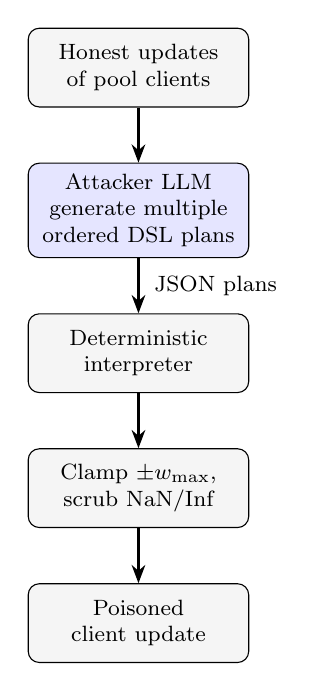
\begin{tikzpicture}[
    node distance=0.7cm and 0.7cm,
    every node/.style={font=\footnotesize},
    box/.style={draw, rounded corners, align=center, minimum height=1.0cm, minimum width=2.8cm, fill=gray!8, inner sep=4pt},
    llmbox/.style={box, fill=blue!10},
    arr/.style={-Stealth, thick}
]
\node[box] (obs) {Honest updates\\of pool clients};
\node[llmbox, below=of obs] (att) {Attacker LLM\\generate multiple\\ordered DSL plans};
\node[box, below=of att] (interp) {Deterministic\\interpreter};
\node[box, below=of interp] (clamp) {Clamp $\pm w_{\max}$,\\scrub NaN/Inf};
\node[box, below=of clamp] (poison) {Poisoned\\client update};

\draw[arr] (obs) -- (att);
\draw[arr] (att) -- node[right,xshift=2pt]{JSON plans} (interp);
\draw[arr] (interp) -- (clamp);
\draw[arr] (clamp) -- (poison);
\end{tikzpicture}
\caption{Attacker action pipeline.}
\vspace{2mm}
\small The LLM never edits weights; it only emits a JSON plan of primitive operators that a fixed interpreter applies.
\label{fig:pipeline}
\end{figure}

\begin{table}[!ht]
\caption{Attack operator DSL with 10 primitives.}
\label{tab:ops}
\centering
\small
\begin{tabular}{@{}ll@{}}
\toprule
\textbf{Operator} & \textbf{Effect} \\
\midrule
\texttt{scale} & multiply targeted weights by a factor \\
\texttt{sign\_flip} & negate the top fraction (by magnitude) \\
\texttt{add\_gaussian\_noise} & add $\mathcal{N}(0,\sigma^2)$ per coordinate \\
\texttt{mask} & zero a fraction (largest / smallest / random) \\
\texttt{clip} & clamp values to $\pm v$ \\
\texttt{add\_constant} & additive shift \\
\texttt{permute} & randomly shuffle coordinates \\
\texttt{scale\_neurons} & scale a fraction of highest-norm output rows \\
\texttt{blend\_random} & convex-blend with scaled random noise, $\alpha$ \\
\texttt{quantize} & round to a fixed step size \\
\bottomrule
\end{tabular}
\vspace{1mm}

\small Each operator applies to \texttt{"all"}, a layer group, or a full parameter key.
\end{table}



\subsection{Reward Design}
\label{sec:rewards}
\begin{equation}
R_{\mathrm{att}} = \alpha \cdot \mathrm{clip}\!\left(\frac{\Delta A}{\tau_a}, -0.5, 1.5\right) + \beta S - \gamma M - \delta C + \zeta D,
\label{eq:attacker_reward}
\end{equation}
where $\Delta A = \mathrm{acc}_{t-1} - \mathrm{acc}_t$ is the induced accuracy drop and $\tau_a$ (\texttt{target\_accuracy\_drop}, default 0.20) is the target drop for the \texttt{untargeted\_degrade} goal. $S \in [0,1]$ is a continuous stealth term, the mean over the chosen clients of $1-\hat p(\mathrm{malicious})$, where $\hat p$ maps the training-time detector's confidence to a soft probability via $\hat p = 0.5 \pm 0.5\cdot\mathrm{confidence}$ (sign depending on its flag). $M$ is the fraction of chosen clients whose plan was malformed or unparseable. $C=(n_{\mathrm{used}}-1)/(|P|-1)$ is a use-fewer-clients penalty, zero for a single-client attack. $D\in[0,1]$ is a diversity bonus, $D = 1 - \overline{\cos}$, the complement of the mean pairwise cosine similarity between the chosen clients' \emph{perturbation vectors} $(w^{\text{poison}}_i - w^{\text{benign}}_i)$, active only when $n_{\mathrm{used}}>1$. This rewards coordinated, distinct multi-client attacks over identical Sybil-like clones, which would otherwise present as an easy-to-catch, high-pairwise-cosine signal. Default weights, $\alpha{=}1.0$, $\beta{=}0.5$, $\gamma{=}1.0$, $\delta{=}0.3$, $\zeta{=}0.2$ (Table~\ref{tab:hparams}). The reward is continuous rather than binary because the GRPO advantage in Eq.~\eqref{eq:advantage} collapses to zero whenever every sampled rollout in a group receives the same reward, a failure mode particularly likely in the small, near-binary action space of choosing which clients to poison.

\subsection{GRPO Training}
\label{sec:rl}
Each attack round yields one exactly computable scalar reward, so a separate per-token value model offers limited benefit; GRPO samples $G$ completions, scores them with the verifiable reward, and normalizes the scores within the group without a critic network \cite{grpo}. For a group of $G$ sampled completions $\{o_1,\dots,o_G\}$ with rewards $\{r_1,\dots,r_G\}$, the group-normalized advantage is
\begin{equation}
A_i = \frac{r_i - \mathrm{mean}(r)}{\mathrm{std}(r) + \epsilon}.
\label{eq:advantage}
\end{equation}
When $\mathrm{std}(r) < \epsilon$, every $A_i$ is set to 0 and the fraction of such groups is logged as a stalled-gradient signal. The policy is updated by
\begin{equation}
\mathcal{L} = \frac{1}{G}\sum_{i=1}^{G}\Big[-A_i \cdot \overline{\log \pi_\theta(o_i)} + \beta \cdot \overline{\mathrm{KL}}(\pi_\theta \,\|\, \pi_{\mathrm{ref}})_i\Big],
\label{eq:grpo-loss}
\end{equation}
where the bar denotes the mean over generated tokens, $\pi_{\mathrm{ref}}$ is the frozen base model (LoRA adapter disabled) evaluated with the k3 KL estimator, and $\beta$ controls the KL penalty. Because updates are single-iteration, no PPO-style clipping term is required \cite{schulman2017ppo}.

\begin{figure}[!ht]
\centering
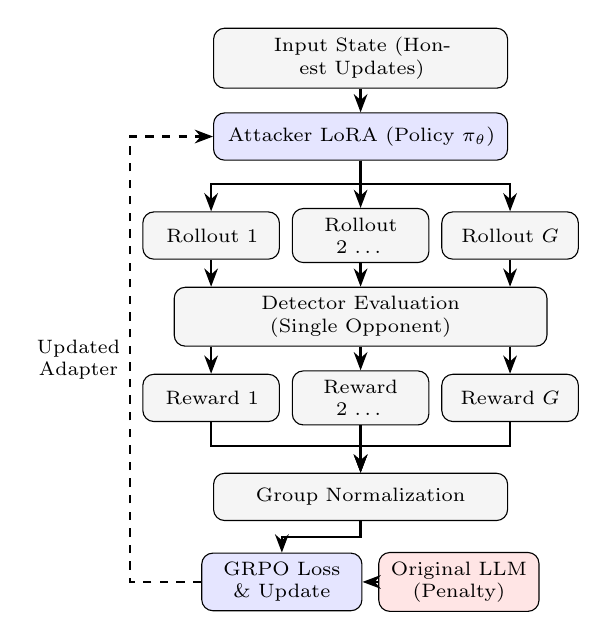
\begin{tikzpicture}[
    node distance=0.4cm and 0.15cm,
    every node/.style={font=\scriptsize},
    box/.style={draw, rounded corners, align=center, minimum height=0.6cm, text width=1.5cm, fill=gray!8},
    llmbox/.style={box, fill=blue!10},
    refbox/.style={box, fill=red!10},
    arr/.style={-Stealth, thick},
    dasharr/.style={-Stealth, thick, dashed}
]

\node[box, text width=3.5cm] (state) {Input State (Honest Updates)};
\node[llmbox, text width=3.5cm, below=0.3cm of state] (policy) {Attacker LoRA (Policy $\pi_\theta$)};

% Rollouts
\node[box, below=0.6cm of policy] (rmid) {Rollout 2 \dots};
\node[box, left=0.15cm of rmid] (r1) {Rollout 1};
\node[box, right=0.15cm of rmid] (rg) {Rollout $G$};

% Eval
\node[box, text width=4.5cm, below=0.3cm of rmid] (eval) {Detector Evaluation (Single Opponent)};

% Reward
\node[box, below=0.3cm of eval] (rewmid) {Reward 2 \dots};
\node[box, left=0.15cm of rewmid] (rew1) {Reward 1};
\node[box, right=0.15cm of rewmid] (rewg) {Reward $G$};

% Group norm
\node[box, text width=3.5cm, below=0.6cm of rewmid] (norm) {Group Normalization};

% Update
\node[llmbox, text width=1.8cm, below=0.4cm of norm, xshift=-1cm] (update) {GRPO Loss\\\& Update};

% Reference
\node[refbox, text width=1.8cm, right=0.2cm of update] (ref) {Original LLM\\(Penalty)};

% Connections
\draw[arr] (state) -- (policy);

\draw[arr] (policy.south) -- +(0,-0.3) -| (r1.north);
\draw[arr] (policy.south) -- (rmid.north);
\draw[arr] (policy.south) -- +(0,-0.3) -| (rg.north);

\draw[arr] (r1) -- (r1 |- eval.north);
\draw[arr] (rmid) -- (eval.north);
\draw[arr] (rg) -- (rg |- eval.north);

\draw[arr] (rew1 |- eval.south) -- (rew1);
\draw[arr] (eval.south) -- (rewmid);
\draw[arr] (rewg |- eval.south) -- (rewg);

\draw[arr] (rew1.south) -- +(0,-0.3) -| (norm.north);
\draw[arr] (rewmid.south) -- (norm.north);
\draw[arr] (rewg.south) -- +(0,-0.3) -| (norm.north);

\draw[arr] (norm.south) -- +(0,-0.2) -| (update.north);
\draw[arr] (ref) -- (update);

% Loop back
\draw[dasharr] (update.west) -- +(-0.9,0) |- (policy.west) node[pos=0.25, left, align=center] {Updated\\Adapter};

\end{tikzpicture}
\caption{GRPO training loop for the attacker policy.}
\vspace{2mm}
\small Only the attacker LoRA adapter is updated; the detector opponent supplies a stochastic confidence signal used solely to compute the reward.
\label{fig:grpo-loop}
\end{figure}

\subsection{Stochastic Opponent Scoring and League Training}
\label{sec:opponent-scoring}
A critical failure mode in this setting is \emph{zero-advantage collapse} (Figure~\ref{fig:grpo-loop}). If the detector opponent responds deterministically, every sampled rollout of the attacker may face the same response; once the attacker is clearly winning or losing, all $G$ rewards converge and $A_i \to 0$ in Eq.~\eqref{eq:advantage}, eliminating the gradient. We therefore sample the frozen detector opponent at temperature $\tau=0.7$ during scoring, so different attacker rollouts face varied responses and reward spread is restored. The committed action that advances the environment still uses the opponent's greedy response at $\tau=0$, keeping the transition deterministic and reproducible. Training proceeds in phases: the attacker trains against a frozen opponent snapshot until it accumulates \texttt{success\_streak} consecutive committed wins (default 3) or \texttt{max\_phase\_rounds} elapse without one (default 4000), after which the opponent snapshot is refreshed. With probability \texttt{league\_prob} (default 0.25), the attacker instead faces a randomly selected past opponent snapshot from a stored league, which reduces overfitting to any single detector generation.

\begin{algorithm}[ht]
\caption{Zero-Touch LLM-Directed Attacker Training via GRPO}
\label{alg:attacker}
\begin{algorithmic}[1]
\State \textbf{Input:} Initial global model $G_0$, budget $b$, target drop $\tau_a$, frozen base LLM $\pi_{\mathrm{ref}}$
\State Initialize attacker LoRA policy $\pi_\theta$ and detector opponent league $\mathcal{L}$
\For{round $t = 1, 2, \dots, T$}
    \State Distribute $G_{t-1}$ to clients and obtain honest local updates $\Delta_i$
    \State Attacker observes $o_t^A$ (normalized statistics of $\Delta_i$ for controllable pool $P$)
    \State Sample $G$ completions $a_1, \dots, a_G \sim \pi_\theta(\cdot|o_t^A)$
    \For{each completion $j \in \{1,\dots,G\}$}
        \State Parse $a_j$ to extract selected clients (up to $b$) and DSL plans
        \State Apply plans to benign weights via deterministic interpreter
        \State Clamp updates to $\pm w_{\max}$ and scrub NaN/Inf values
        \State Server aggregates poisoned and honest updates to form $G_t^{(j)}$
        \State Evaluate accuracy $\mathrm{acc}_t^{(j)}$ and accuracy drop $\Delta A^{(j)}$
        \State Sample opponent detector from $\mathcal{L}$ at temperature $\tau=0.7$
        \State Compute stealth score $S^{(j)}$ from detector confidence
        \State Compute reward $R_{\mathrm{att}}^{(j)}$ using Eq.~\eqref{eq:attacker_reward}
    \EndFor
    \State Compute group-normalized advantages $A_j$ for $j=1,\dots,G$ using Eq.~\eqref{eq:advantage}
    \State Update $\pi_\theta$ by maximizing GRPO objective (Eq.~\eqref{eq:grpo-loss})
    \If{success streak reached}
        \State Update opponent league $\mathcal{L}$ with current detector snapshot
    \EndIf
\EndFor
\end{algorithmic}
\end{algorithm}

\section{Experimental Setup}
\label{sec:setup}

\subsection{Implementation}
The framework is implemented in PyTorch. LLM loading, LoRA injection, and GRPO training use the Unsloth library on top of Hugging Face PEFT and Transformers; no external RL trainer (e.g., TRL) dependency is required, since GRPO is implemented directly against the environment's verifiable reward.

\subsection{Dataset and Partitioning}
We evaluate the framework across three distinct datasets and specific client scenarios. The data is partitioned using the FLTrust-style non-IID bias-$q$ scheme \cite{fltrust} (default $q=0.5$). Table~\ref{tab:scenarios} details the evaluation settings.

\begin{center}
\captionof{table}{Evaluation Datasets and Client Scenarios}
\label{tab:scenarios}
\small
\begin{tabular}{@{}lcc@{}}
\toprule
\textbf{Dataset} & \textbf{Total Clients} & \textbf{Poisoned Clients} \\
\midrule
Fashion MNIST & 5 & 1 \\
MNIST & 10 & 5 \\
5G-NIDD & 20 & 5 \\
\bottomrule
\end{tabular}
\end{center}

The attacker's controllable pool represents a strict minority in the 20-client setting (small-budget run), and half the federation in the 10-client setting (large-budget run, detailed in Section~\ref{sec:run-config}).

\subsection{Model and LLM Configuration}
Table~\ref{tab:llmconfig} summarizes the policy backbone. The attacker is a single LoRA adapter over a shared, frozen \texttt{Qwen2.5-7B-Instruct} base \cite{lora2022}; a separate detector adapter over the same frozen base is used only as a training-time opponent (Section~\ref{sec:opponent-scoring}) and is not part of the evaluated attacker.

\begin{center}
\captionof{table}{Model and LLM configuration.}
\label{tab:llmconfig}
\small
\begin{tabular}{@{}ll@{}}
\toprule
\textbf{Component} & \textbf{Configuration} \\
\midrule
Global model & MLP, 970 parameters (MNIST) \\
LLM base & \texttt{Qwen2.5-7B-Instruct} (Unsloth), shared, frozen \\
Precision & bf16 LoRA \\
Evaluated policy & 1$\times$ LoRA adapter (\texttt{attacker}) \\
Attention impl. & eager (default), sdpa (optional) \\
\bottomrule
\end{tabular}
\end{center}

\subsection{Training Hyperparameters}
Table~\ref{tab:hparams} lists the GRPO, schedule, and reward hyperparameters used in all runs unless otherwise noted.

\begin{center}
\captionof{table}{GRPO, schedule, and attacker-reward hyperparameters.}
\label{tab:hparams}
\small
\begin{tabular}{@{}lc@{}}
\toprule
\textbf{Hyperparameter} & \textbf{Value} \\
\midrule
Group size $G$ & 4 \\
KL penalty $\beta$ & 0.02 \\
Learning rate & $1.0\times10^{-5}$ \\
Opponent scoring temperature $\tau$ & 0.7 \\
Committed-action temperature & 0.0 (greedy) \\
Success streak (opponent refresh) & 3 consecutive wins \\
Max phase rounds (cap) & 4000 \\
Target accuracy drop $\tau_a$ & 0.20 (train) / 0.10 (eval) \\
Reward weights $\alpha,\beta,\gamma,\delta,\zeta$ & 1.0, 0.5, 1.0, 0.3, 0.2 \\
Non-IID bias $q$ & 0.5 \\
\bottomrule
\end{tabular}
\end{center}

\subsection{Defense Panel}
\label{sec:defense-panel}
The trained attacker adapter is benchmarked, unmodified, against four independently evolving, fixed defenses drawn from the published literature; none of these defenses is proposed in this paper, and every one receives the exact same committed poisoned update set each round (Section~\ref{sec:benchmark-protocol}). Table~\ref{tab:defenses} summarizes the panel.

\begin{center}
\captionof{table}{Defense panel.}
\label{tab:defenses}
\small
\begin{tabular}{@{}p{1.5cm}p{6cm}@{}}
\toprule
\textbf{Defense} & \textbf{Mechanism} \\
\midrule
FLTrust & Trust score $= \mathrm{ReLU}(\cos(\Delta_i, g_0))$ against a clean-root-set reference update $g_0$, surviving deltas rescaled to $\|g_0\|$ and trust-weighted averaged \cite{fltrust}. \\
Multi-Krum & Keeps the $m{=}n{-}f$ clients with smallest summed squared distance to their $n{-}f{-}2$ closest neighbors \cite{krum}. \\
DnC & Projects centered updates onto the top right singular vector of the client matrix, drops the $c \cdot m$ clients with largest squared projection \cite{dnc}. \\
DeFL & Tracks a per-layer Federated Gradient Norm Vector, detects Critical Learning Periods from its round-over-round rise, and votes a client malicious via an adaptive per-layer outlier threshold (MOUD) \cite{defl}. \\
\bottomrule
\end{tabular}
\vspace{1mm}

\small Every entry is a fixed, published mechanism used only as an evaluation target; none is proposed in this paper, and the attacker studied here never trains against, or adapts to, any of them.
\end{center}

Multi-Krum and DnC require an assumed upper bound $f$/$m$ on the number of malicious clients (a hyperparameter, not per-round ground truth); we default it to the evaluation poison budget, clamped to a benign majority, $f \le \lfloor (N-1)/2 \rfloor$. FLTrust additionally requires a small clean root dataset (default 100 samples) that the server fine-tunes the global model on for one local epoch each round to obtain its trust reference.

\subsection{Benchmark Protocol}
\label{sec:benchmark-protocol}
Each benchmark round, the environment samples the controllable pool's honest updates, and the trained attacker LLM (temperature 0.7) produces \emph{one} client selection and DSL plan against the reference (no-defense) accuracy. That single set of poisoned updates is then fed, unmodified, to every defense in the panel, each evolving its own global model and returning its own accept/reject verdicts (Figure~\ref{fig:benchmark}). Holding the attack fixed while only the defense varies is what makes the resulting comparison attributable to the defense rather than to attack variance. We report, per defense, ground-truth detection metrics, true-positive rate (TPR/recall), false-positive rate (FPR), precision, and F1, and robustness metrics, final and mean test accuracy, mean accuracy drop versus the clean baseline, the fraction of rounds a poisoned client evaded detection (\texttt{thru}), and attack success rate (\texttt{succ}).

\begin{figure}[!h]
\centering
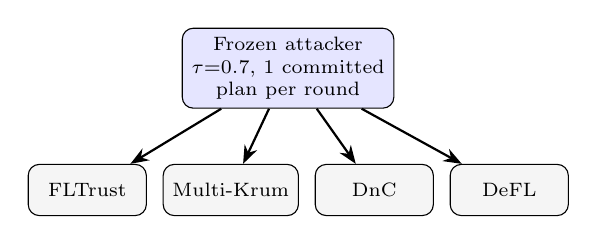
\begin{tikzpicture}[
    node distance=0.7cm and 0.2cm,
    every node/.style={font=\scriptsize},
    box/.style={draw, rounded corners, align=center, minimum height=0.65cm, minimum width=1.5cm, fill=gray!8},
    llmbox/.style={box, fill=blue!10},
    arr/.style={-Stealth, thick}
]
\node[llmbox] (att) {Frozen attacker\\$\tau{=}0.7$, 1 committed\\plan per round};
\node[box, below=0.7cm of att, xshift=-2.55cm] (d1) {FLTrust};
\node[box, right=0.2cm of d1] (d2) {Multi-Krum};
\node[box, right=0.2cm of d2] (d3) {DnC};
\node[box, right=0.2cm of d3] (d4) {DeFL};

\draw[arr] (att) -- (d1);
\draw[arr] (att) -- (d2);
\draw[arr] (att) -- (d3);
\draw[arr] (att) -- (d4);
\end{tikzpicture}
\caption{Benchmark protocol.}
\label{fig:benchmark}
\end{figure}

\section{Results and Discussion}
\label{sec:results}

\textit{The results in this section report two benchmark runs of the trained attacker adapter against the defense panel at two different poison budgets. They are single runs at single configurations, not yet averaged over seeds or intermediate budgets, and should be read as preliminary evidence of the mechanism's behavior rather than a fully replicated finding (Section~\ref{sec:limitations}).}

\subsection{Benchmark Run Configurations}
\label{sec:run-config}
\textbf{Run A (small budget).} $n=50$ attack rounds, a clean baseline accuracy of $0.782$, the \texttt{untargeted\_degrade} goal with target accuracy drop $\tau_a = 0.10$, and an evaluation poison budget of $b=2$ of a $n_{\mathrm{compromisable}}=5$-client pool, a strict minority consistent with Section~\ref{sec:threat}. Multi-Krum's and DnC's assumed-malicious-count hyperparameter was set to the true budget, $f=m=2$.

\textbf{Run B (large budget).} $n=20$ attack rounds, a clean baseline accuracy of $0.897$, the same $\tau_a=0.10$ goal, and a poison budget of $b=10$ clients per round held as an exact quota, half of $N=20$. This is deliberately \emph{outside} the strict-minority regime: Byzantine-robust guarantees such as Multi-Krum's own bound, $n \geq 2f+3$, generally require the malicious fraction to stay strictly below $1/2$, so Run B is a boundary stress test of what happens once that assumption is no longer satisfied. Because Multi-Krum's and DnC's assumed-malicious-count hyperparameter is clamped to $\lfloor (N-1)/2\rfloor = 9$, both were handed $f=m=9$ against a true budget of $10$, a one-client underestimate that arises mechanically from the clamp itself. In both runs the attacker adapter was frozen and sampled at temperature 0.7; every defense in the panel evolved its own global model against the identical committed attack each round.

\begin{table*}[t]
\caption{Run A defense-panel results.}
\label{tab:results}
\centering
\small
\begin{tabular}{@{}lccccccccc@{}}
\toprule
\textbf{Defense} & \textbf{Detect\%} & \textbf{FPR} & \textbf{Prec} & \textbf{F1} & \textbf{Final acc.} & \textbf{Mean acc.} & \textbf{Acc. drop} & \textbf{thru} & \textbf{succ} \\
\midrule
FLTrust & 75.0\% & 71.7\% & 0.10 & 0.18 & 0.772 & 0.778 & $+0.004$ & 46.0\% & 0.0\% \\
DeFL & 91.0\% & 7.3\% & 0.58 & 0.71 & 0.338 & 0.451 & $+0.332$ & 18.0\% & 56.0\% \\
DnC & 66.0\% & 3.8\% & 0.66 & 0.66 & 0.787 & 0.741 & $+0.042$ & 68.0\% & 6.0\% \\
Multi-Krum & 100.0\% & 0.0\% & 1.00 & 1.00 & 0.784 & 0.784 & $-0.001$ & 0.0\% & 0.0\% \\
\bottomrule
\end{tabular}
\vspace{1mm}

\small Evaluated for 50 attack rounds, baseline accuracy 0.782, target drop $\tau_a=0.10$, and poison budget $b=2$ of 5.
\end{table*}

\begin{table*}[t]
\caption{Run B defense-panel results.}
\label{tab:results-run-b}
\centering
\small
\begin{tabular}{@{}lccccccccc@{}}
\toprule
\textbf{Defense} & \textbf{Detect\%} & \textbf{FPR} & \textbf{Prec} & \textbf{F1} & \textbf{Final acc.} & \textbf{Mean acc.} & \textbf{Acc. drop} & \textbf{thru} & \textbf{succ} \\
\midrule
FLTrust & 95.0\% & 77.0\% & 0.55 & 0.70 & 0.891 & 0.891 & $+0.006$ & 5.0\% & 5.7\% \\
DeFL & 1.0\% & 2.0\% & 0.33 & 0.02 & 0.064 & 0.072 & $+0.825$ & 100.0\% & 100.0\% \\
DnC & 41.5\% & 48.5\% & 0.46 & 0.44 & 0.065 & 0.054 & $+0.843$ & 100.0\% & 100.0\% \\
Multi-Krum & 53.5\% & 36.5\% & 0.59 & 0.56 & 0.426 & 0.537 & $+0.359$ & 100.0\% & 95.9\% \\
\bottomrule
\end{tabular}
\vspace{1mm}

\small Evaluated for 20 attack rounds, baseline accuracy 0.897, target drop $\tau_a=0.10$, and poison budget $b=10$ (exact quota).
\end{table*}

\begin{figure}[t]
\centering
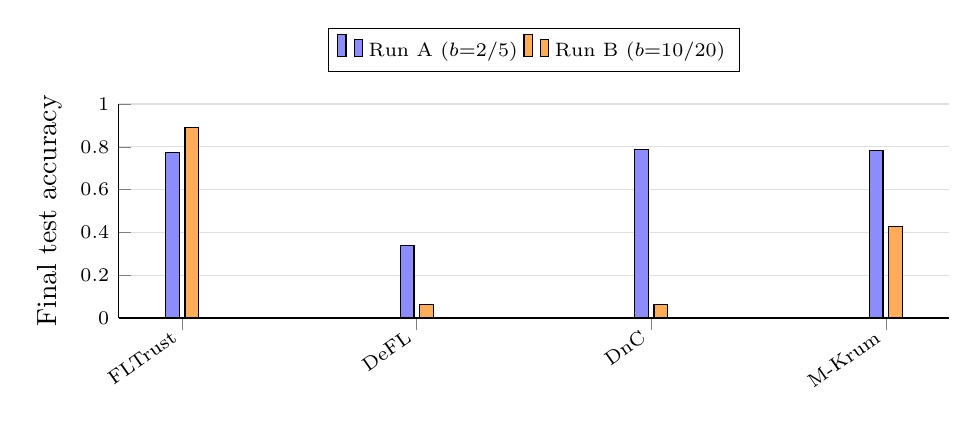
\begin{tikzpicture}
\begin{axis}[
    ybar, bar width=5pt,
    width=\linewidth, height=4.3cm,
    ylabel={Final test accuracy},
    symbolic x coords={FLTrust,DeFL,DnC,M-Krum},
    xtick=data,
    x tick label style={font=\scriptsize,rotate=35,anchor=east},
    y tick label style={font=\scriptsize},
    ymin=0, ymax=1.0,
    legend style={font=\scriptsize,at={(0.5,1.15)},anchor=south,legend columns=-1},
    enlarge x limits=0.09,
    axis lines*=left,
    ymajorgrids, grid style={gray!25},
]
\addplot[fill=blue!45] coordinates {(FLTrust,0.772) (DeFL,0.338) (DnC,0.787) (M-Krum,0.784)};
\addplot[fill=orange!65] coordinates {(FLTrust,0.891) (DeFL,0.064) (DnC,0.065) (M-Krum,0.426)};
\legend{Run A ($b{=}2/5$), Run B ($b{=}10/20$)}
\end{axis}
\end{tikzpicture}
\caption{Final test accuracy per defense.}
\vspace{2mm}
\small Evaluated under the identical, frozen attacker at each budget. Run A baseline 0.782; Run B baseline 0.897 (dashed references omitted for clarity).
\label{fig:results-bar}
\end{figure}

\subsection{The Small-Budget Regime}
At $b{=}2$ of 5, a strict minority of the federation, Multi-Krum achieves near-perfect results, 100\% detection, 0\% FPR, 0.784 final accuracy, 0\% attack success, despite never having seen this attacker during training: the attacker's committed perturbations were, every round, distant enough from the honest bulk under Multi-Krum's nearest-neighbor distance score to be excluded outright. FLTrust and DnC show a second pattern, moderate binary detection (75\% and 66\%) at high or moderate FPR, yet negligible realized damage ($+0.004$ and $+0.042$ mean accuracy drop), because both apply a continuous re-weighting or projection to every surviving update rather than a hard accept/reject filter, so even rounds where a poisoned client's flag is missed contribute little to the aggregate. DeFL inverts this pattern: the \emph{highest} detection rate of any defense in the panel (91\%) and the best F1 (0.71), yet the most damage (final accuracy 0.338, 56\% attack success), because its Critical-Learning-Period gating makes its filtering strength non-uniform round to round, and a handful of missed early rounds leave the global model in a degraded state that later, correctly-flagged rounds cannot undo. Per-round detection metrics alone did not predict which defense actually protected the model.

\subsection{The Large-Budget Regime}
At $b{=}10$ of 20, half the federation, the picture changes sharply and unevenly (Table~\ref{tab:results-run-b}, Figure~\ref{fig:results-bar}). DeFL's detection rate falls from Run A's best-in-panel 91\% to exactly 0\%, and its final accuracy (0.064), mean drop ($+0.825$), and attack success (100\%) show a near-total collapse; DnC degrades almost as completely (41.5\% detect, 48.5\% FPR, essentially a coin flip, 100\% attack success). Multi-Krum holds up only partially: its mean accuracy (0.537) is the least damaged of the three collapsing defenses, but a 0.36 absolute drop and 95.9\% attack success remain. We read this as the panel failing close to where its own theory says it should rather than as a flaw the attack specifically exploited: Multi-Krum's bound $n \geq 2f+3$ is violated outright at $f=10$, $n=20$, and both Multi-Krum's and DnC's assumed-malicious-count hyperparameter is mechanically clamped to $f=9$, one client short of the truth, because $\lfloor (N-1)/2\rfloor=9$ is the largest value the clamp permits at $N=20$.

What did \emph{not} collapse is the more surprising result. FLTrust (0.891 final accuracy, $+0.006$ drop) remains close to the clean baseline even with half the federation compromised. Unlike Multi-Krum and DnC, FLTrust does not depend on an assumed malicious-count hyperparameter: it anchors every update to a clean root-set reference independent of how many clients are compromised. This suggests that robustness at large poison budgets tracks whether a defense's assumptions scale with the malicious fraction, not merely its detection accuracy at a single, smaller budget.

\subsection{Limitations}
\label{sec:limitations}
These results come from two single runs at two fixed configurations. First, neither run has been repeated across seeds or at intermediate budgets between $b{=}2$ and $b{=}10$, so the shape of the transition between the two regimes is unknown. Second, Run B could not isolate the mismatched-assumption question (the one-client clamp underestimate) from the budget-exceeds-guarantee question for Multi-Krum and DnC; a deliberate ablation holding the true budget fixed while varying only the assumed count is still needed. Third, the divergence between detection metrics and realized protection observed for DeFL is diagnosed here from the mechanism's design, not from an ablation isolating its Critical-Learning-Period trigger. Fourth, the benchmark harness runs no honest-FL recovery interlude between attack rounds, so any defense that misses even a small number of early rounds accumulates damage for the remainder of the run, which stresses worst-case persistence and may overstate real-world damage relative to a deployment that periodically re-trains or resets. Fifth, both runs operate over a compact, 970-parameter MLP; per-layer statistics of this size may not transfer to substantially larger architectures without redesigning the feature extractor and the DSL's targeting granularity.

\section{Conclusion}
\label{sec:conclusion}
We presented a zero-touch, LLM-directed FL attacker that learns, via GRPO over a verifiable reward, which clients to poison and how to compose primitive weight operators against them, without a hand-authored attack template. Benchmarked unmodified against four independently evolving, fixed defenses from the published literature across two poison-budget regimes, the attacker was fully neutralized by Multi-Krum and FLTrust at a strict-minority budget, and drove DeFL and DnC toward near-total success once its budget reached half the federation, while FLTrust held the global model close to baseline at that same larger budget. Per-round detection metrics did not reliably predict realized protection. Future work will replicate both runs across seeds, sweep intermediate budgets, run a mismatched-assumption ablation for Multi-Krum/DnC, extend the global model beyond a single compact MLP, and study Sybil client creation and targeted (backdoor) attack goals against the same panel.

\begin{thebibliography}{00}

\bibitem{fedavg}
H. B. McMahan, E. Moore, D. Ramage, S. Hampson, and B. A. y Arcas, ``Communication-efficient learning of deep networks from decentralized data,'' in \emph{Proc. 20th Int. Conf. Artificial Intelligence and Statistics (AISTATS)}, 2017, pp. 1273--1282.

\bibitem{bagdasaryan2020}
E. Bagdasaryan, A. Veit, Y. Hua, D. Estrin, and V. Shmatikov, ``How to backdoor federated learning,'' in \emph{Proc. 23rd Int. Conf. Artificial Intelligence and Statistics (AISTATS)}, 2020, pp. 2938--2948.

\bibitem{bhagoji2019}
A. N. Bhagoji, S. Chakraborty, P. Mittal, and S. Calo, ``Analyzing federated learning through an adversarial lens,'' in \emph{Proc. 36th Int. Conf. Machine Learning (ICML)}, 2019, pp. 634--643.

\bibitem{byzantine}
D. Yin, Y. Chen, R. Kannan, and P. Bartlett, ``Byzantine-robust distributed learning: Towards optimal statistical rates,'' in \emph{Proc. 35th Int. Conf. Machine Learning (ICML)}, 2018, pp. 5650--5659.

\bibitem{krum}
P. Blanchard, E. M. El Mhamdi, R. Guerraoui, and J. Stainer, ``Machine learning with adversaries: Byzantine tolerant gradient descent,'' in \emph{Advances in Neural Information Processing Systems}, vol. 30, 2017.

\bibitem{dnc}
V. Shejwalkar and A. Houmansadr, ``Manipulating the Byzantine: Optimizing model poisoning attacks and defenses for federated learning,'' in \emph{Proc. Network and Distributed System Security Symp. (NDSS)}, 2021.

\bibitem{fltrust}
X. Cao, M. Fang, J. Liu, and N. Z. Gong, ``FLTrust: Byzantine-robust federated learning via trust bootstrapping,'' in \emph{Proc. Network and Distributed System Security Symp. (NDSS)}, 2021.

\bibitem{foolsgold}
C. Fung, C. J. M. Yoon, and I. Beschastnikh, ``The limitations of federated learning in sybil settings,'' in \emph{Proc. 23rd Int. Symp. Research in Attacks, Intrusions and Defenses (RAID)}, 2020, pp. 301--316.

\bibitem{defl}
G. Yan \emph{et al.}, ``DeFL: Defending against model poisoning attacks in federated learning via critical learning periods awareness,'' in \emph{Proc. AAAI Conf. Artificial Intelligence}, 2023.

\bibitem{fang2020}
M. Fang, X. Cao, J. Jia, and N. Z. Gong, ``Local model poisoning attacks to Byzantine-robust federated learning,'' in \emph{Proc. 29th USENIX Security Symp.}, 2020, pp. 1605--1622.

\bibitem{xie2020fallofempires}
C. Xie, O. Koyejo, and I. Gupta, ``Fall of empires: Breaking Byzantine-tolerant SGD by inner product manipulation,'' in \emph{Proc. 36th Conf. Uncertainty in Artificial Intelligence (UAI)}, 2020, pp. 261--270.

\bibitem{baruch2019little}
G. Baruch, M. Baruch, and Y. Goldberg, ``A little is enough: Circumventing defenses for distributed learning,'' in \emph{Advances in Neural Information Processing Systems}, vol. 32, 2019.

\bibitem{wang2020attackoftails}
H. Wang, K. Sreenivasan, S. Rajput, H. Vishwakarma, S. Agarwal, J.-y. Sohn, K. Lee, and D. Papailiopoulos, ``Attack of the tails: Yes, you really can backdoor federated learning,'' in \emph{Advances in Neural Information Processing Systems}, vol. 33, 2020, pp. 16070--16080.

\bibitem{cao2022mpaf}
X. Cao and N. Z. Gong, ``MPAF: Model poisoning attacks to federated learning based on fake clients,'' in \emph{Proc. IEEE/CVF Conf. Computer Vision and Pattern Recognition Workshops (CVPRW)}, 2022, pp. 3396--3404.

\bibitem{grpo}
Z. Shao, P. Wang, Q. Zhu, R. Xu, J. Song, X. Bi, H. Zhang, M. Zhang, Y. K. Li, Y. Wu, and D. Guo, ``DeepSeekMath: Pushing the limits of mathematical reasoning in open language models,'' 2024, arXiv:2402.03300.

\bibitem{schulman2017ppo}
J. Schulman, F. Wolski, P. Dhariwal, A. Radford, and O. Klimov, ``Proximal policy optimization algorithms,'' 2017, arXiv:1707.06347.

\bibitem{ouyang2022instructgpt}
L. Ouyang \emph{et al.}, ``Training language models to follow instructions with human feedback,'' in \emph{Advances in Neural Information Processing Systems}, vol. 35, 2022, pp. 27730--27744.

\bibitem{lora2022}
E. J. Hu, Y. Shen, P. Wallis, Z. Allen-Zhu, Y. Li, S. Wang, L. Wang, and W. Chen, ``LoRA: Low-rank adaptation of large language models,'' in \emph{Proc. Int. Conf. Learning Representations (ICLR)}, 2022.

\bibitem{dubey2024llama3}
A. Dubey \emph{et al.}, ``The Llama 3 herd of models,'' 2024, arXiv:2407.21783.

\bibitem{nguyen2022flame}
T. D. Nguyen \emph{et al.}, ``FLAME: Taming backdoors in federated learning,'' in \emph{Proc. 31st USENIX Security Symp.}, 2022, pp. 1415--1432.

\end{thebibliography}

\end{document}